
%(BEGIN_QUESTION)
% Copyright 2007, Tony R. Kuphaldt, released under the Creative Commons Attribution License (v 1.0)
% This means you may do almost anything with this work of mine, so long as you give me proper credit

If the feedwater control valve for a boiler is placed in manual and then given a ``step-change'' in position, the effect on steam drum water level will look something like this:

$$\includegraphics[width=15.5cm]{i01798x01.eps}$$

It seems quite normal that water level would ramp up at a constant rate, liquid level control being a characteristically {\it integrating} process.  However, that initial ``shrink'' in water level is quite unexpected to anyone unfamiliar with boiler controls.

\vskip 10pt

The shrink results from the addition of more (cool) feedwater to the boiler, which immediately reduces boiler temperature, causing some of the steam bubbles rising in the tubes and drum to re-condense into water.  This artificially drops the steam drum level a bit before it begins to rise from the added water.

Boiler shrink is a problem for drum level control, because it makes the controller ``think'' the water level is moving {\it the wrong direction}.  Explain how this physical effect negatively impacts feedback control, and determine whether the impact is more pronounced in a {\it single-element} or a {\it two-element} feedwater control system.

\underbar{file i01798}
%(END_QUESTION)





%(BEGIN_ANSWER)

By initially moving the ``wrong direction'' in response to a change in feedwater flow, the drum level feedback signal to the controller actually constitutes {\it positive} feedback rather than negative.  The 180$^{o}$ phase shift of proportional action combined with the 180$^{o}$ phase shift of boiler ``shrink'' makes 360$_{o}$.

\vskip 10pt

Follow-up question: integrating processes such as liquid level typically respond well to aggressive proportional control action (proportional bands of 10\% or less!), but not in this case.  How would you recommend tuning the level controller in a boiler feedwater control system, given the effect of ``shrink?''

%(END_ANSWER)





%(BEGIN_NOTES)

Anyone who has ever added cold water to a pot of boiling pasta/water knows firsthand what ``shrink'' is and what causes it!

\vskip 10pt

Two-element feedwater control systems are less impacted by shrink than single-element.

\vskip 10pt

Follow-up answer: instead of relying on high controller gain, the gain must be tempered and more integral action incorporated into the PID tuning.

%INDEX% Control, PID tuning: step change (output) revealing negative lead
%INDEX% Physics, heat and temperature: boiler ``shrink''

%(END_NOTES)


